\subsection*{Report 2}

	The second exercise simulated sound travelling from a source to a target, with first and second order reflections from the walls being included. The MATLAB script used can be found on page \pageref{matlab_1.2}. A damping factor of 0.5 was used to allow the signals to decrease over time, as it would in reality. An impulse response was sent as the source, and from the simulated received pulses the room channel impulse response was calculated through a convolution of the original impulse response and the simulated received response. Figure \ref{figure:1_2} shows that both the received signal and calculated response are the same, as expected.
	
	\begin{figure}[H] 
		\centering
		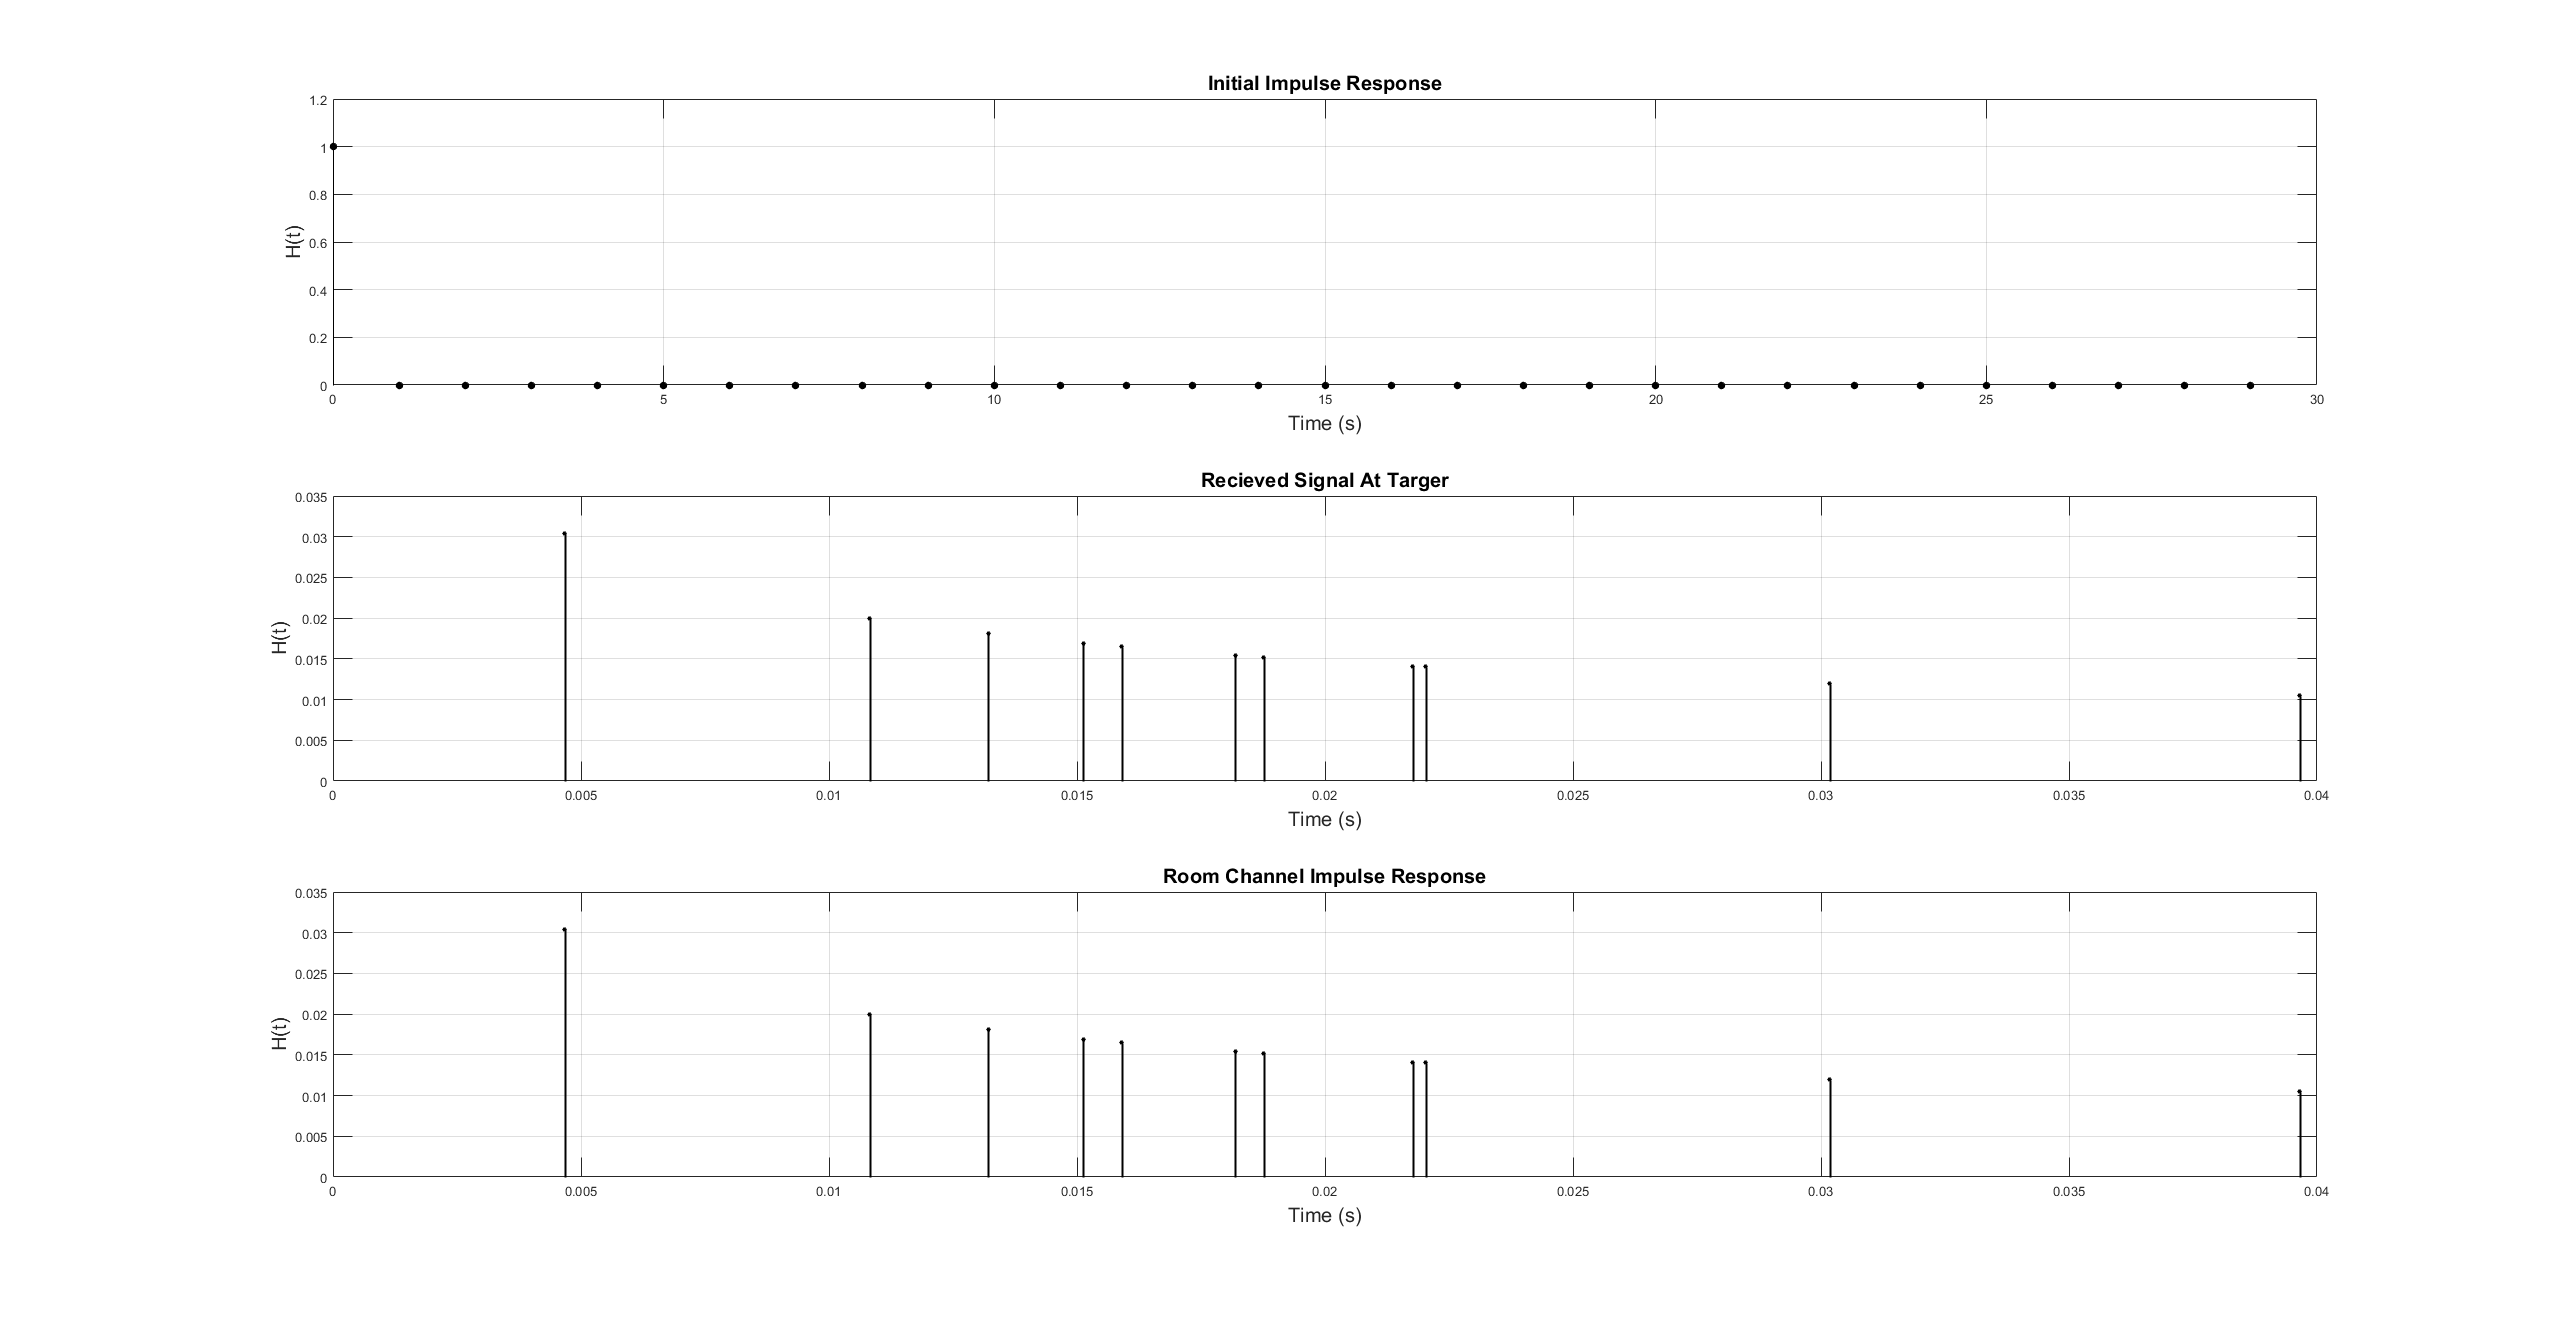
\includegraphics[width=\textwidth]{1.2.png}
		\caption{Room Channel Impulse Response \& Reflected Signals}
		\label{figure:1_2}
	\end{figure}